\subsection{M.PC.EAC - Estimated at Completion}

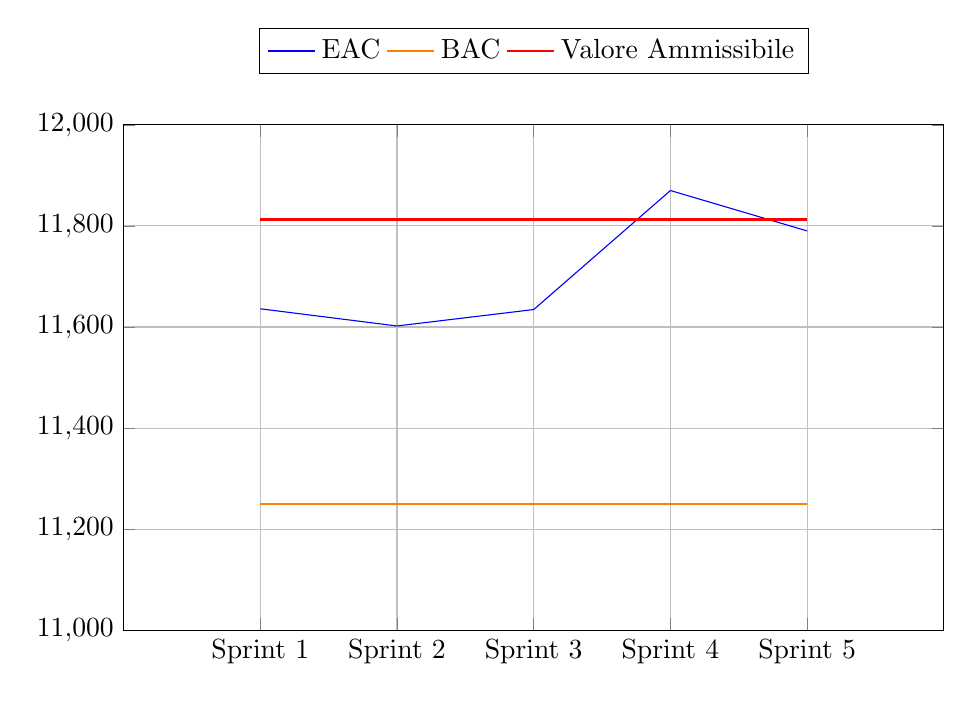
\begin{tikzpicture}
    \begin{axis}[
        width=12cm, height=8cm,
        ymin=11000, ymax=12000,
        xmin=0, xmax=6,
        xtick={1, 2, 3, 4, 5},
        xticklabels={Sprint 1, Sprint 2, Sprint 3, Sprint 4, Sprint 5},
        xlabel={},
        ylabel={},
        grid=major,
        scaled ticks=false,
        legend style={at={(0.5,1.1)}, anchor=south, legend columns=-1},
    ]
    \addplot[color=blue] coordinates {(1, 11636) (2, 11602) (3, 11634.5) (4, 11870) (5, 11790)};
    \addlegendentry{EAC}
    \addplot[orange, thick] coordinates {(1, 11250) (5, 11250)};
    \addlegendentry{BAC}
    \addplot[red, thick] coordinates {(1, 11812.5) (5, 11812.5)};
    \addlegendentry{Valore Ammissibile}
    \end{axis}
\end{tikzpicture}
\subsubsection{RTB}
Il grafico mostra che l'Estimated at Completion, a eccezione dello \glossario{sprint} 4, rimane all'interno del valore ammissibile, indicando una gestione efficiente dei costi di progetto. 
Questo significa che eventuali deviazioni nei costi sostenuti e nel valore guadagnato durante gli \glossario{sprint} 
sono state compensate nel corso del progetto, mantenendo il controllo sulla spesa complessiva